\RequirePackage{shellesc}
\immediate\write18{cd ..; tex braids_code.dtx}
\documentclass{article}

\usepackage{tikz}
\usetikzlibrary{braids,calc}

\newcommand{\braidcode}{}
\begin{document}
\begin{center}
  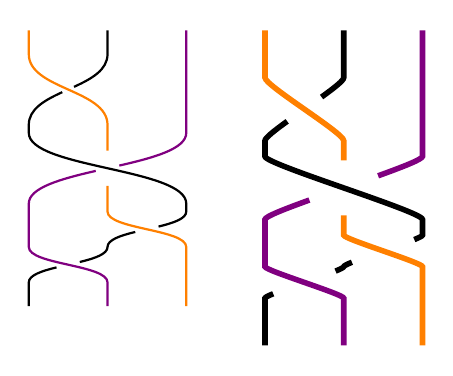
\begin{tikzpicture}[
    every braid/.style={
      braid/strand 1/.style=orange,
      braid/strand 3/.style=violet,
    }]
    \pic[thick] (braid1) at (0,0) {braid={s_1 s_{1,3} s_{1-3}}};
    \pic[
    line width=2pt,
    braid/.cd,
    border height=5mm,
    gap=.15,
    control factor=.2,
    nudge factor=.1,
    ] (braid2) at (3,0) {braid={s_1  s_{1,3} s_{1-3}}};
  \end{tikzpicture}
\end{center}


\begin{center}
  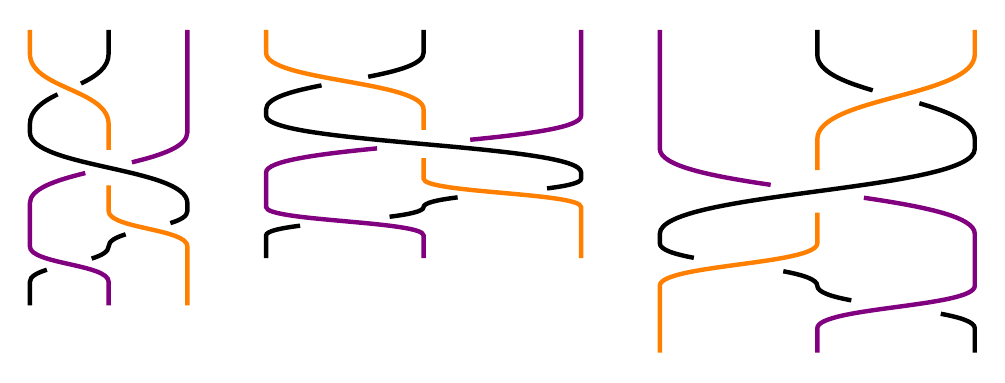
\begin{tikzpicture}[
    every braid/.style={
      ultra thick,
      braid/gap=.1,
      braid/strand 1/.style=orange,
      braid/strand 3/.style=violet,
    }]
    \pic (braid1) at (0,0) {braid={s_1 s_{1,3} s_{1-3}}};
    \pic[
    braid/.cd,
    width=2cm,
    crossing height=.8cm,
    ] (braid3) at (3,0) {braid={s_1  s_{1,3} s_{1-3}}};
    \pic[
    braid/.cd,
    width=-2cm,
    crossing height=1.2cm,
    ] (braid3) at (12,0) {braid={s_1  s_{1,3} s_{1-3}}};
  \end{tikzpicture}
\end{center}


\end{document}
